%%%%%%%%%%%%%%%%% Begin
%%%%% Este código es especial para agregar secciones en capítulos sin número, se usa en la introducción y en las conclusiones. 
\renewcommand{\altname}{Conclusiones}
\lhead[\fancyplain{}{}]%
      {\fancyplain{}{\bfseries \altname}}
\addchap{\altname}
%%%%%%%%%%%%%%%%% End
%%%%%%%%%%%%%%%%% Empezar a escribir abajo de esta línea. 
En este trabajo nos enfocamos en el estudio de las propiedades de las estructuras formadas por materia oscura. Hemos realizo diversas simulaciones, cada una una con una cosmología diferente. Se busco tener Universos con cosmologías planas, sub-críticas y super-críticas. Las propiedades que se estudiaron de las diversas simulaciones fueron el número de halos, la masa de los halos, el radio que contiene la mitad de la masa, el radio donde se alcanza la velocidad máxima de rotación, así como la velocidad máxima de rotación y la dispersión de velocidades.

Lo primero que podemos notar en la figura \ref{fig:Conc_TotalHalos} es que la simulaciones con una cosmología sub-crítica ($\Omega < 1$) comienzan a formar estructura mucho antes que el resto. Las simulaciones $\Omega_0 = 309$ $\Omega_\lambda=0$ y $\Omega_0=0.1545$ $\Omega_\lambda=0.691$ vemos que las estructuras empiezan a formarse en $z=25$ y en $\Omega_0=0.309$ $\Omega_\lambda=0.3455$ las vemos en $z=22$. Estas mismas cosmologías alcanzan la mayor cantidad de halos a lo largo de su evolución, la simulación $\Omega_0 = 309$ $\Omega_\lambda=0$ forman un máximo de $28,192$ halos en $z=2.33$ y en $z=0$ se termina teniendo $22,136$ halos, la simulación $\Omega_0 = 0.1545$ $\Omega_\lambda=0.691$ forman un máximo de $28,044$ halos en $z=2.33$ y en $z=0$ se termina teniendo $21,911$ y la simulación $\Omega_0 = 0.309$ $\Omega_\lambda=0.3455$ forman un máximo de $27,483$ en halos $z=2$ y en $z=0$ se termina teniendo $21,821$ halos. Mientras que el resto de las cosmologías empiezan a formar sus halos entre $z=13$ y $z=17$, donde el máximo de halos está entre $25,968$ y $26,242$ el cual se alcanza en $z=1.5$ y en $z=0$ en rango de halos esta entre $20,883$ y $20,777$.

\begin{figure}[H]
      \centering
      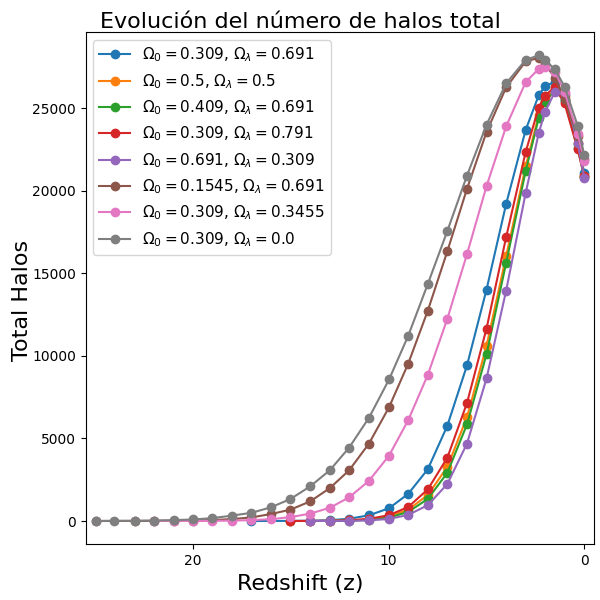
\includegraphics[scale=0.5]{Conc/TotalHalos_Conc.png}
      \caption[Evolución del total de halos para todas las cosmologías]{El número total de halos a lo largo de la evolución del sistema para las diferentes cosmologías que se realizaron}
      \label{fig:Conc_TotalHalos}
\end{figure}

Si nos enfocamos ahora en la masa, podemos apreciar que las cosmologías con un incremento en $\Omega_0$ forman las estructuras más masivas. En la figura \ref{fig:Conc_Mass} podemos ver que la cosmología $\Omega_0=0.691$ $\Omega_\lambda=0.309$ tiene la masa media más alta a lo largo de toda la simulación, alcanzando la masa de $10^{11.09}M_\odot$, mientras que la cosmología $\Omega_0=0.1545$ $\Omega_\lambda=0.691$ vemos que las estructuras que forman, tienen la masa media más baja de las cosmologías, alcanzando la masa de $10^{10.45} M_\odot$. También podemos notar que la desviación estándar, para $z$ altos, en las simulaciones con cosmologías sub-críticas es mayor que en el resto de las cosmologías lo que nos dice que tenemos una mayor variación en la masa de las estructuras encontradas, en cambio para $z$ cercanas al cero, la desviación se acerca al mismo valor.
\begin{figure}[H]
      \centering
      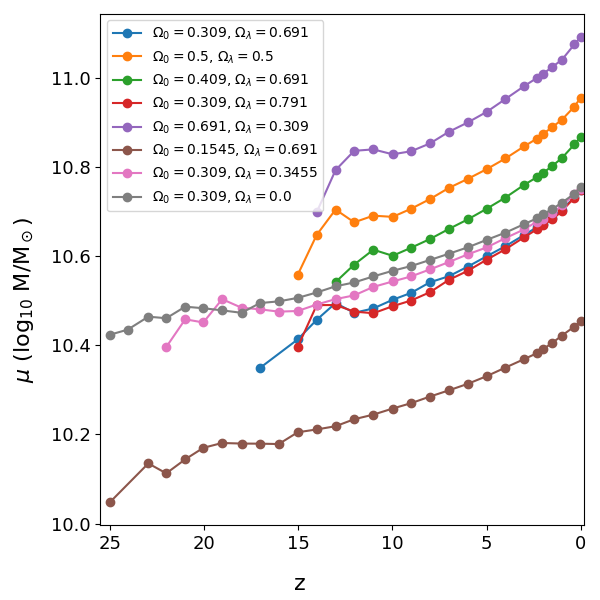
\includegraphics[width=0.48\linewidth]{Conc/MassMean_Conc.png}
      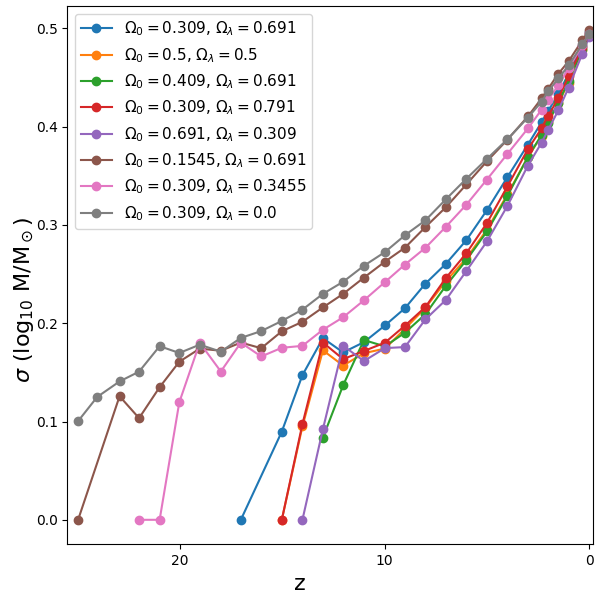
\includegraphics[width=0.48\linewidth]{Conc/MassStd_Conc.png}
      \caption[Evolución de la desviación y media de la masa de los halos para todas las cosmologías]{La desviación y media de la masa de los halos a lo largo de la evolución del sistema para las diferentes cosmologías que se realizaron}
      \label{fig:Conc_Mass}
\end{figure}

Lo que podemos observar con el radio que contiene a la mitad de la masa en la figura \ref{fig:Conc_HalfMassRad} es que el radio medio sigue un comportamiento similar, crecen a un ritmo similar de manera que es difícil distinguirlos, pero las cosmologías con un incremento en $\Omega_0$ tiene un radio medio ligeramente mayor al resto alcanzando $10^{1.5}$ kpc en $z=0$, mientras que las cosmologías sub-críticas forman estructuras ligeramente más pequeñas, teniendo una media de $10^{1.41}$ kpc en z=0. Mientras, la desviación estándar se comporta de forma similar a la masa, donde las cosmologías sub-críticas tienen una variación mayor entre $z=10 y z=1$ pero en $z=0$ se acercan a un mismo valor. Por lo tanto, el radio que contiene la mitad de la masa no es bueno en cuanto a su media, mientras que la variación de masas nos sirve en $z$ intermedios.

\begin{figure}[H]
      \centering
      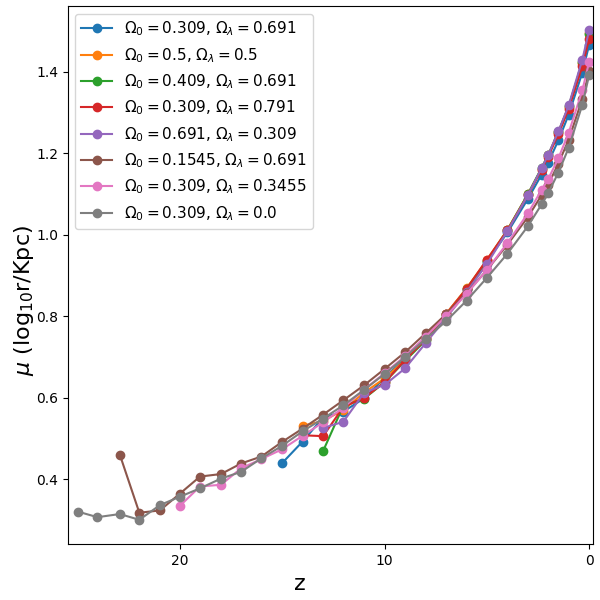
\includegraphics[width=0.48\linewidth]{Conc/HalfMassRad_Mean_Conc.png}
      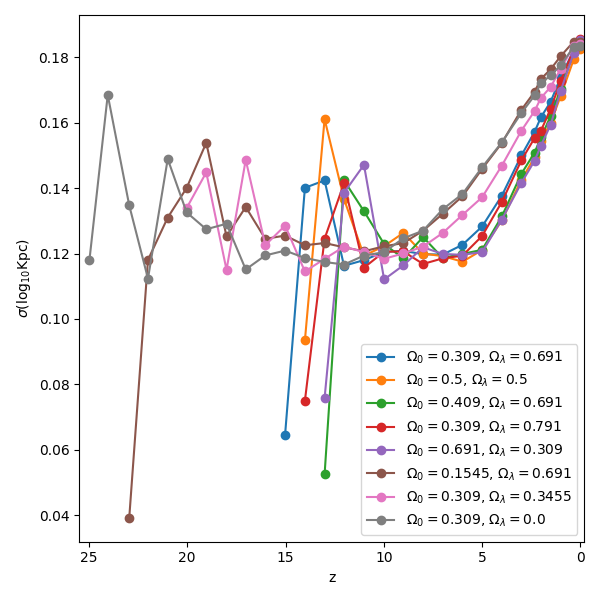
\includegraphics[width=0.48\linewidth]{Conc/HalfMassRad_Std_Conc.png}
      \caption[Evolución de la desviación y media del radio que contiene la mitad de la masa de los halos para todas las cosmologías]{La desviación y media del radio que contiene la mitad de la masa de los halos a lo largo de la evolución del sistema para las diferentes cosmologías.}
      \label{fig:Conc_HalfMassRad}
\end{figure}

{\morado Seguimos con el radio en el cual se alcanza la velocidad circular máxima. En la figura} \ref{fig:Conc_VMaxRad} vemos que los Universos con un incremento $\Omega_0$ forman estructuras con radio medio con un pequeño incremento, alcanzando los $30.52$ kpc en $z=0$ mientras que en los Universos sub-críticos, las estructuras tienen los radios medios mas pequeños donde el radio medio alcanza los $21.99$ kpc. Mientras que la desviación estándar se comporta de manera similar, donde tenemos una desviación de $18.73$ kpc cuando incrementamos $\Omega_0$ y $10.78$ kpc en los Universos sub-críticos.

\begin{figure}[H]
      \centering
      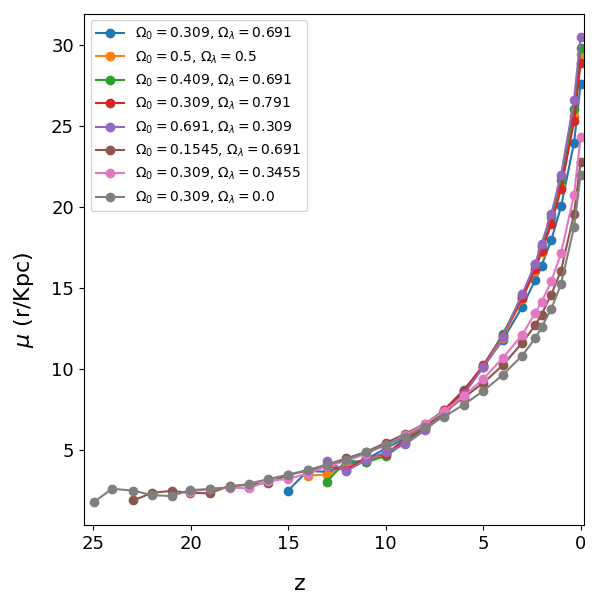
\includegraphics[width=0.48\linewidth]{Conc/VMaxRad_Mean_Conc.png}
      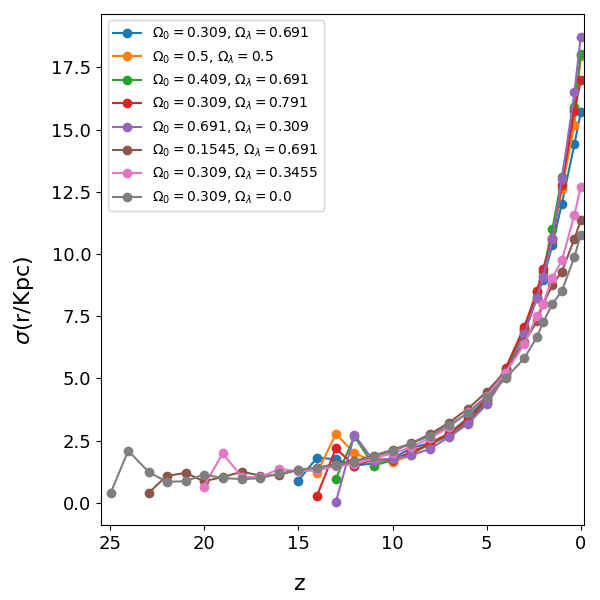
\includegraphics[width=0.48\linewidth]{Conc/VMaxRad_Std_Conc.png}
      \caption[Evolución de la desviación y media del radio donde se alcanza la velocidad circular máxima de los halos para todas las cosmologías]{La desviación y media del radio donde se alcanza la velocidad máxima de los halos a lo largo de la evolución del sistema para las diferentes cosmologías que se realizaron}
      \label{fig:Conc_VMaxRad}
\end{figure}

Cuando observamos la velocidad máxima de los halos en la figura \ref{fig:Conc_VelMax}, podemos notar que entre más grande sea el $\Omega_0$, los halos que se forman alcanzan una mayor velocidad. En la cosmología $\Omega_0 = 0.691$ $\Omega_\lambda = 0.309$ alcanza una velocidad de $220$km/s en $z=12$ y en $z=0$ bajo a una velocidad de $106.07$km/s y en la cosmología  $\Omega_0 = 0.1545$, $\Omega_\lambda = 0.691$ se tiene una velocidad de $126.67$km/s en $z=21$ y llega en $z=0$ a $57.84$km/s. Viendo la desviación, es difícil asegurar los efectos de modificar los parámetros cosmológicos, tan solo se vemos que se ve afectado por los cambios en $\Omega_0$.

\begin{figure}[H]
      \centering
      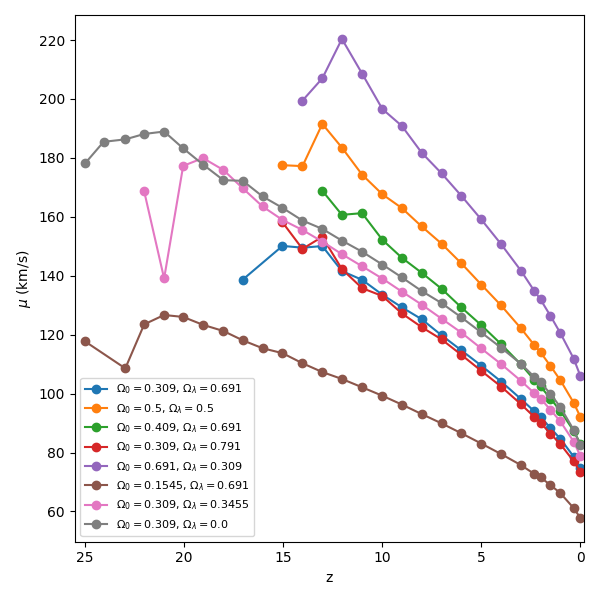
\includegraphics[width=0.48\linewidth]{Conc/VelMax_Mean_Conc.png}
      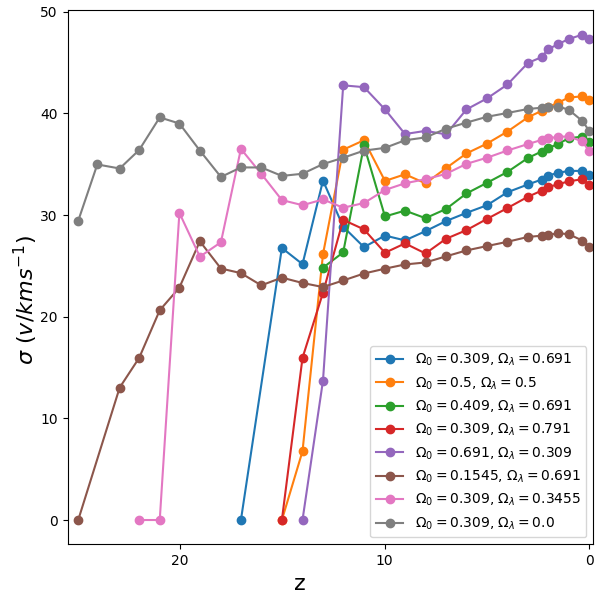
\includegraphics[width=0.48\linewidth]{Conc/VelMax_Std_Conc.png}
      \caption[Evolución de la desviación y media de la velocidad máxima de los halos para todas las cosmologías]{La desviación y media de la velocidad máxima de los halos a lo largo de la evolución del sistema para las diferentes cosmologías que se realizaron}
      \label{fig:Conc_VelMax}
\end{figure}

En la figura \ref{fig:Conc_VelDisp} podemos apreciar que la dispersión de velocidades se ve afectado con el aumento de $\Omega_0$, donde podemos ver que en la cosmología $\Omega_0 = 0.691$, $\Omega_\lambda = 0.309$ alcanza una velocidad de $125.60$km/s en $z=12$ y en $z=0$ bajo a una velocidad de $54.03$km/s y en la cosmología  $\Omega_0 = 0.1545$, $\Omega_\lambda = 0.691$ se tiene una velocidad de $71.90$km/s en $z=21$ y llega en $z=0$ a $27.33$km/s. 

\begin{figure}[H]
      \centering
      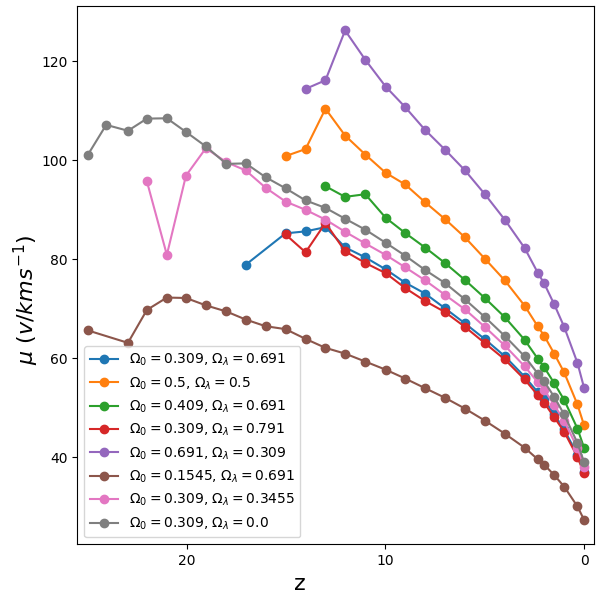
\includegraphics[width=0.48\linewidth]{Conc/VelDisp_Mean_Conc.png}
      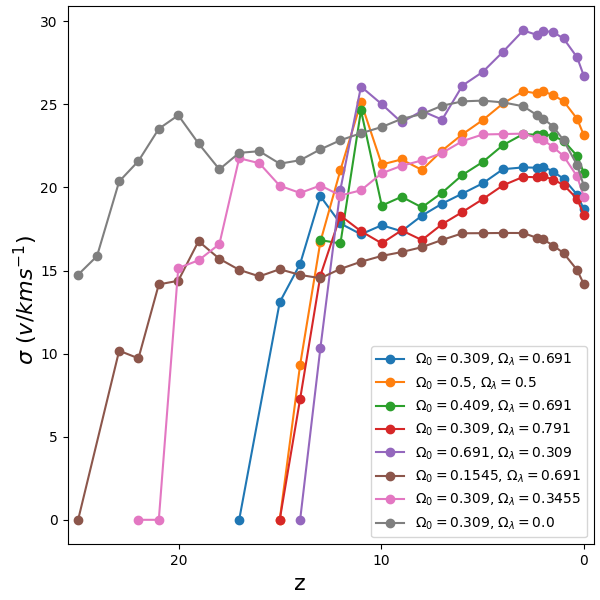
\includegraphics[width=0.48\linewidth]{Conc/VelDisp_Std_Conc.png}
      \caption[Evolución de la desviación y media de la dispersión de velocidades los halos para todas las cosmologías]{La desviación y media de la dispersión de velocidades de los halos a lo largo de la evolución del sistema para las diferentes cosmologías que se realizaron}
      \label{fig:Conc_VelDisp}
\end{figure}

Podemos ver que las velocidades se ven alteradas por los cambios en $\Omega_0$, mientra que el tamaño y la masa se ven afectadas por los cambios en $\Omega_0$ y en el tipo de cosmología, ya sea un Universos cerrado, abierto o plano. De lo que nos dimos cuenta fue que el radio no es un buen parámetro ya que su comportamiento es difícil de distinguir entre cosmologías.  Pudimos observar que las cosmologías sub-críticas forman estructuras más pequeñas y menos densas que el resto de las cosmologías y que la cosmología $\Omega_0 = 0.691$, $\Omega_\lambda = 0.309$ tiene grandes estructuras de gran masa que alcanzan grandes velocidades, es decir que el aumento de $\Omega_0$ for estructuras de mayor masa y con una mayor dinámica.

Con este trabajo podemos inferir como es el comportamiento en la evolución de un Universo según sea sus densidades de materia y energía. Esto nos ayuda a poder inferir que tipo de Universo es en el que vivimos ya que podemos usar las observaciones y compararlas con resultados como estos para inferir las densidades del Universo.
%%%%% Este código es especial para agregar secciones en capítulos sin número, se usa en la introducción y en las conclusiones. Se pueden agregar tantas secciones como sea necesario, solo copiar las lineas entre los 
% (desde Begin hasta End). 
%\renewcommand{\altname}{Puntos L1,L2 y L3}%%%%% Solo necesitas %editar esta línea con el título de la sección
%\lhead[\fancyplain{}{}]%
%      {\fancyplain{}{\bfseries \altname}}
%\addsec{\altname}
%%%%%%%%%%%%%%%%% End
 

%%%%%%%%%%%%%%%%%%%%%%%%%%% Begin
%%%%%%%%%%%%%% No escribir  después de estas líneas. 
%%%%%%%%%%%%%% Este texto debe permanecer al final de este archivo!!!
\lhead[\fancyplain{}{}]%
      {\fancyplain{}{\bfseries\rightmark}}
%%%%%%%%%%%%%%%%%%%%%%%%%%% End
